\section{Integrerade Kretsar (IC)}
\index{integrerada kretsar}
\label{integrerade kretsar}

\subsection{Allmänt om IC}
\index{integrerad krets}
\index{IC}

Att integrera betyder att samla till en enhet, det kan vara komponenter,
funktioner eller verksamheter.
Integration kan ske på olika nivåer och i många olika sammanhang.

Med integration avses här integration av komponenter för elektroniska
strömkretsar.
Särskilt halvledarelement av olika slag samt resistorer och kondensatorer med
små värden kan framställas med små dimensioner.
Många komponenter kan då samlas i samma hölje.

Komponenter inom ett hölje, avsedda för en viss funktion kallas
\emph{integrerad krets} (eng. \emph{Integrated Circuit -- IC}).

Komponenterna i en IC kan i sin tur vara del av komponenterna en hel strömkrets.
Redan inom höljet kan komponenter kopplas samman för en viss funktion eller som
en del av strömkretsen.
Skrymmande eller effektkrävande komponenter, såsom induktorer, transformatorer
och så vidare får emellertid inte plats, varför även yttre kopplingar behövs.
Det kan också behövas flera IC i en strömkrets -- kanske med innehåll för en
annan funktion.

\subsection{Integrationsgrad}

En integrerad krets är uppbyggd på en basplatta av halvledarmaterial -- ett chip.
På plattan framställs, med fototeknik eller etsning, kompletta eller nästan
kompletta dioder, transistorer, resistorer och kondensatorer.
Metoden, som kallas planarteknik, medger att många komponenter kan få plats på
samma platta.

Den snabba utvecklingen av produktionsmetoder för integrerade kretsar gör
alltmer avancerade system möjliga och dessutom på allt mindre utrymme.
Med avseende på integrationsgrad används följande begrepp.

\begin{tabular}{lp{6cm}}
SSI & Small Scale Integration innebär något 10-tal halvledare på samma chip. \\
MSI & Medium Scale Integration innebär något 100-tal halvledare på ett chip. \\
LSI & Large Scale integration innebär något 10000-tal halvledare på ett chip. \\
VLSI & Very Large Scale Integration innebär 100000 eller fler halvledare. \\
\end{tabular}

\subsection{Olika slags integrerade kretsar}

Det finns stora sortiment av både standardiserade och speciella IC, varav det
finns två huvudtyper:
\begin{itemize}
  \item digitala integrerade kretsar
  \item analoga integrerade kretsar.
\end{itemize}

\subsection{Digitala IC}

Digitala IC arbetar som framgår av namnet med digitala signalnivåer.
De enklaste typerna innehåller en eller flera digitala grindar (se avsnitt
\ref{digitala kretsar}).
Genom att koppla samman grindar kan man skapa kretsar för ett visst ändamål.
I början av 70-talet byggdes komplicerade system av grindar i SSI- och
MSI-teknik.
Ett sådant system är emellertid inte flexibelt eftersom eventuella ändringar
måste göras ''hårdvarumässigt''.
Det innebär att kopplingsledningar måste ändras, kanske hela kretsar bytas ut
och så vidare.

I dagens digitala system används IC i form av en mikroprocessor eller till och
med flera.
En mikroprocessor är en avancerad krets som kan programmeras (konfigureras)
mjukvarumässigt inte bara för ett ändamål utan för många olika.
I system med mikroprocessorer behövs också minnesfunktioner.
Mikroprocessorn är hjärtat i en dator.
Styrd av ett program (mjukvaran) kontrollerar den kringutrustningar med uppgift
att inhämta och avge information -- att kommunicera.

\subsection{Analoga IC}

Analoga IC arbetar med analoga signalnivåer, det vill säga spänningar och
strömmar med kontinuerligt varierande nivåer och frekvenser.
En analog IC kan även arbeta med digitala signaler.

Analoga IC innehåller en eller flera balanserade förstärkare samt olika slags
hjälpkretsar.
Med yttre komponenter kan en analog IC ges olika förstärkning och frekvensgång.
Med ett gemensamt namn kallas dessa förstärkare för operationsförstärkare
(OP-amp).
Operationsförstärkare utförs vanligen i SSI- eller möjligen MSI-teknik.

\subsection{Kombinerade och speciella IC}

Utöver standardiserade IC finns kombinerade och speciella IC.
Exempel på speciella digitala IC är sådana för telekommunikationsändamål.
Ett annat exempel på digitala IC är sådana för signalbehandling, såväl på HF
som LF-nivå.
Exempel på speciella analoga IC är sådana för radiokommunikationsändamål.

Bortsett från vissa skrymmande komponenter och manöverdon kan numera till
exempel en IC innehålla en komplett radiomottagare.
Ett annat exempel på speciella analoga IC är sådana för hörapparater.
Genom programmering anpassas de för det personliga behovet.

\subsection{Utvecklingen}

Det kan sägas hur ofta som helst.
Genom den fantastiska utvecklingen av mikroelektronik öppnas även för
radioamatören möjligheter som tidigare inte var tänkbara.

Denna utveckling har vidgat utrymmet för den experimentella verksamhet som
amatörradio i grunden innebär.
Hobbyn får sålunda med tiden en allt större teknisk spännvidd.

\subsection{Aktuell litteratur}

Ökat teknikomfång inom amatörradio ställer motsvarande krav på litteratur.
På senare tid inbegripes även digitalteknik.
Mest av utrymmesskäl behandlas i denna faktabok digitaltekniken mycket
kortfattat, men ändå så mycket som nämns i CEPT-rekommendationen T/R 61-02.
För djupare studium hänvisas till andra läromedel samt till
leverantörskataloger.

\section{Operationsförstärkare}
\textbf{
HAREC a.\ref{HAREC.a.2.8.3}\label{myHAREC.a.2.8.3}
}
\index{operationsförstärkare}
\index{op-amp}

\emph{Operationsförstärkare} (eng. \emph{operational amplifier}), ofta kallad
för \emph{op-amp} är en integrerad kretstyp som har hög förstärkning.
Istället för att ha enbart en ingång så har den två, en positiv
och en negativ, och operationsförstärkaren förstärker skillnaden mellan den
positiva och negativa signalen. Förstärkningen i en modern
operationsförstärkare kan vara i storleksordningen en miljon gånger.
De två mest grundläggande kopplingarna är komparator respektive negativt
återkopplad förstärkare.

\subsection{Komparator}

I en \emph{komparator} används den höga förstärkningen för att få även små
spänningsskillnader att ge ett stort utslag.
Med referensspänningen på den negativa ingången och insignalen på den positiva
ingången, kommer utgången att vara så hög den kan vara när ingången har högre
spänning än referensspänningen.
Omvänt kommer den vara så låg den kan vara när spänningsnivån på ingången är
lägre än referensspänningen.

Det är enkelt att ändra utgångens egenskaper genom att växla signaler mellan
positiv och negativ ingång på operationsförstärkaren.

\subsection{Negativ återkoppling och förstärkare}

En operationsförstärkare som har en negativ återkoppling, det vill säga där
signal från utgången matas tillbaka till den negativa ingången, kommer att
försöka driva utgången så att spänningsskillnaden mellan den positiva och
negativa ingången jämnas ut.
Det finns en rik uppsättning kopplingar som bygger på denna jämvikt, där
operationsförstärkaren arbetar i ett linjärt driftsområde.

Denna jämvikt gör också att en snabb diagnosticering kan göras genom att mäta
spänningen mellan ingångarna.
Om spänningen ligger nära noll fungerar kopplingen förmodligen.
Men om kopplingen är felaktig på något sätt, exempelvis om själva
operationsförstäkaren eller någon komponent i återkopplingen är trasig, kommer
spänningen vara synbart annorlunda och jämvikten finns inte.

\subsubsection{Buffertförstärkare}

Den enklaste linjära kopplingen med en operationsförstärkare är en
buffertförstärkare.
I denna koppling är den negativa ingången direkt kopplad till utgången och
insignalen är kopplad till den positiva ingången.
Med denna koppling kommer operationsförstärkaren försöka få den negativa
ingången, och därmed även utgången, att följa insignalen.
En sådan koppling, där vi får samma spänning på utgången som vi har på
ingången, kallas för en spänningsföljare.
Fördelen med en spänningsföljare är att lasten på utgången kan vara oerhört
mycket högre än vad insignalen skulle kunna driva.
Om utgångsnivån skulle sjunka beroende på lasten, försöker återkopplingen driva
den tillbaka till rätt spänning.

Buffertförstärkaren gör att operationsförstärkaren kan leverera samma spänning
ut, men mot en last på bara något fåtal ohm, det vill säga med mycket större
strömstyrka.
Den relativt höga ingångsimpedansen hos operationsförstärkaren, uppemot en
teraohm, gör att drivsignalen inte påverkas av en lågohmig last.

\subsubsection{Positiv (icke-inverterande) förstärkning med op-amp}
\label{icke-inverterande förstärkning}

En enkel variant av buffertförstärkaren fås när man kopplar in en
spänningsdelare mellan utgången och den negativa ingången, så som illustreras i
bild \ref{fig:BildII2-46}.

\begin{wrapfigure}{R}{0.5\textwidth}
	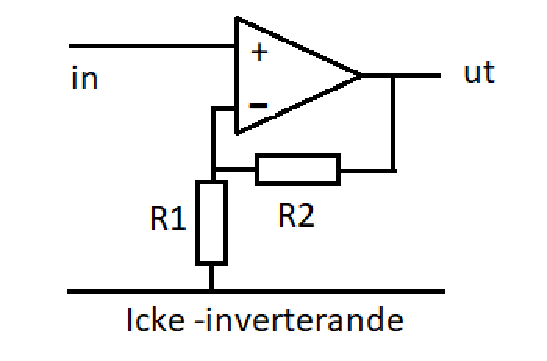
\includegraphics[width=0.5\textwidth]{images/cropped_pdfs/bild_2_2-46.pdf}
	\caption{Icke-inverterande förstärkare}
	\label{fig:BildII2-46}
\end{wrapfigure}

Om förhållandet i spänningsdelaren är 1:10 kommer spänningen på den negativa
ingången att vara en tiondel av spänningen på utgången.
För att behålla jämvikten mellan den positiva och den negativa ingången, kommer
operationsförstärkaren att driva utgången till tio gånger nivån på den positiva
ingången.
Genom att variera förhållandet i spänningsdelaren kan man kontrollera
förstärkningen hos kretsen.
Förstärkningen blir:

\(G = 1+ \dfrac{R_2}{R_1}\)

Genom att koppla en kondensator parallellt över återkopplingsmotståndet
(\(R_2\) i bild \ref{fig:BildII2-46}) kan man skapa en bandbreddsbegränsning
för förstärkaren.
För de högre frekvenserna kommer merparten av strömmen att gå genom
kondensatorn och återkopplingen blir därför frekvensberoende.
Förstärkningen för höga frekvenser sänks mot samma nivå som för en
bufferförstärkare.

Detta är också ett sätt att undvika att kretsen självsvänger vid höga
frekvenser.

\subsubsection{Negativ (inverterande) förstärkning med op-amp}
\label{inverterande förstärkning}
\label{virtuell jord}
\label{jordning!virtuell}

Kopplingen i bild \ref{fig:BildII2-47} ger en negativ förstärkning.

\begin{wrapfigure}{R}{0.5\textwidth}
	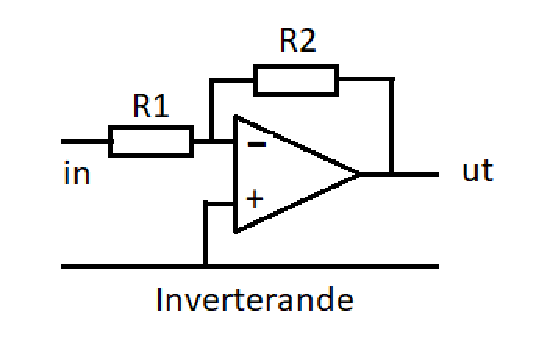
\includegraphics[width=0.5\textwidth]{images/cropped_pdfs/bild_2_2-47.pdf}
	\caption{Inverterande förstärkare}
	\label{fig:BildII2-47}
\end{wrapfigure}

Operationsförstärkaren kommer att balansera den negativa ingången så att den
är på samma potential som jord.
Detta kallas för \emph{virtuell jord}.
Strömmen kommer att gå från ingången till utgången, men ingången kommer se
lasten från ingångsmotståndet \(R_1\) och utgången kommer att mata \(R_2\) mot
jord.
Förstärkningen kommer att vara negativ och proportionell mot kvoten mellan
motståndsvärdena:

\(G = -\dfrac{R_2}{R_1}\)
